\documentclass[a4paper,12pt]{article}
%\RequirePackage[l2tabu,orthodox]{nag}

\usepackage{upreport}
\usepackage{tabularx}

\addbibresource{report.bib}
\title{Noob's Guide to \LaTeX{} 3.14}
\subject{CJJ 310}
\date{\today}

%Nomenclature unit command
\newcommand{\nomunit}[1]{%
\renewcommand{\nomentryend}{\hspace*{\fill}#1}}

\begin{document}
\maketitle
\makecoverpage

\pagestyle{plain}
\thispagestyle{plain}
\pagenumbering{roman}

\begin{center}
\LARGE\textbf{\thetitle}
\end{center}

\section*{Abstract}
\addcontentsline{toc}{section}{Abstract}%
Welcome to The Noob's Guide to \LaTeX. It is a short example of how the scientific content of reports can be typeset within the \LaTeX{} environment. Short examples will illustrate how to typeset tables, figures, equations, chemistry, and references.

Keywords: chemical engineering, reporting, communication
\setcounter{page}{3}

\newpage
\tableofcontents

% \iftotalfigures%
% \newpage%
% \listoffigures%
% \fi

% \iftotaltables%
% %\newpage%
% \listoftables%
% \fi

\newpage

%\chapter*{Nomenclature}
\printnomenclature
\newpage

\pagestyle{plain}
\setcounter{page}{1}
\pagenumbering{arabic}


\section{Introduction} \label{sec:Introduction}
\TeX{} is a low-level programming language created by Donald Knuth in 1977 to typeset documents. The letters of the name represent the
capital Greek letters tau, epsilon, and chi, as \TeX{} is an abbreviation of the Greek word for both ``art" and ``craft". It is therefore pronounced as the fist syllable of ``technical". However, in Afrikaans it's pronounced as the first syllable of ``tegnies".

To simplify the typesetting, Leslie Lamport then developed a macro package called \LaTeX{}, pronounced as ``Lay-tech" or ``Lah-teg". Many later authors have contributed extensions, called \textit{packages} or \textit{styles}, to \LaTeX{}.

Since \LaTeX{} word processing is essentially programming, some users may shy away from the steep learning curve. However, since the formatting is applied consistently throughout the document by commands, it offers an advantage over WYSIWYG (what you see is what you get) word processors like Microsoft Word. The focus thus shifts from superficial formatting issues to writing good content.

A number of online resources that you will definitely need to consult as you continue to use \LaTeX{} are listed below.
The quickest solution is simply to search your question in your favourite search engine with inclusion of the word `latex'.

\begin{itemize}
    \item \href{https://wch.github.io/latexsheet/}{\LaTeX{} Cheat Sheet}
    \item \href{https://tobi.oetiker.ch/lshort/lshort.pdf}{The Not So Short Introduction to \LaTeXe}
    \item \href{https://en.m.wikibooks.org/wiki/LaTeX}{\LaTeX{} wikibook}
    \item \href{http://ftp.leg.uct.ac.za/pub/packages/ctan/info/short-math-guide/short-math-guide.pdf}{Short Math Guide for \LaTeX}
    \item \href{http://tex.stackexchange.com}{\TeX{} Stack Exchange}
\end{itemize}

\section{\LaTeX\ overview}
\subsection{Overleaf}
This guide assumes the use of the online \LaTeX\ editor \href{www.overleaf.com}{Overleaf} which is recommended for beginners. It is analogous to Jupyter for Python code by providing the necessary tools to code and debug a \LaTeX\ document effectively. Students that wish to install a \LaTeX{} distribution to their personal computer for offline document compilation should consult the wikibook for a list of editors such as TeXstudio (note that the installation and use of such editors may require intermediate programming skills).

If this document is open in Overleaf at the moment, the layout consists of three panes and several buttons. The left pane displays the file tree used to compile the document, followed by the code pane and the .pdf preview on the right. The top ribbon contains the buttons as displayed in Table~\ref{tab:overleaf}. 

\begin{table}[htbp]
\centering
\caption{Overleaf tools}
\label{tab:overleaf}
\begin{tabularx}{1.0\textwidth}{lX}
\hlineB{3}
Button & Use\\
\midrule
Menu & Provides the word count, sets the spell check to English (British), and changes the editor theme to \textit{vibrant ink} for working at night\\
Up arrow & Returns to one's project list\\
Review & For writing comments on things to improve\\
Share & For collaborating in real-time\\
Submit & Share your document as an Overleaf template with the world\\
History & Label stable versions of your document as it is developed\\
Chat & For discussions with collaborators \\
\hlineB{3}
\end{tabularx}
\end{table}


If other collaborators are online at the same time, a block with their initial will be displayed next to Review---click it to find where they are in the document. Use the two arrows between the code and preview panes to find a section of code from the preview and \textit{vice versa}. The number of errors in the compiled document are shown in blue, orange or red in increasing severity next to the Recompile button. Clicking it will display them and they are usually humorously straight-forward.

\subsection{The template content}
The Noob's Guide to \LaTeX{} is available on GitHub \href{https://github.com/Franco-Pretorius/Noob-s-Guide-to-LaTeX}{by clicking here}.
The report template on which it is based is available on GitHub from \href{https://github.com/ChemEngUP/ce-up-latex-templates}{Chemical Engineering at UP LaTeX templates}. It can be downloaded as a ZIP file from the green Clone or Download button. To add this template to your Overleaf project list, click New Project, then Upload Project and drag the .zip folder to the window.

This template was written by Carl Sandrock using an offline editor, thus many of the background processes used to generate the document won't be discussed. The source files are listed in Table~\ref{tab:sourceFiles}. Entries listed in \textbf{boldface} are the files one will usually edit. 

\begin{table}[htbp]
\centering
\caption[Template source files]{The source files included in the current departmental \LaTeX\ template with their function. }
\label{tab:sourceFiles}
\begin{tabularx}{1.0\textwidth}{lX}
\hlineB{3}
.gitignore & This file serves only the development of the template by contributors to the project. It may safely be ignored and deleted to compile documents.\\
README.md & This file serves only the development of the template by contributors to the project. It may safely be ignored and deleted to compile documents.\\
biblatex.cfg & This file defines the configuration of the reference list. \\
frontmatter.tex & This file contains the report front matter. Note that the list of tables and figures should be removed.\\
latexmkrc & This file defines the configuration of the reference list.\\
\textbf{report.bib} & This file contains the report references.\\
\textbf{report\_template.tex} & This file contains the main report content.\\
samplefigure.py & This file is used to generate the figure that is given in the 2019 departmental Style Guide. It may be safely ignored and deleted to compile a different report. Note that this code would be run \textit{outside} the \LaTeX\ environment.\\
\textbf{synopsis.tex} & This file contains the report synopsis.\\
upreport.sty & This file defines a number of style related constructs to adhere to the 2019 departmental Style Guide, as well as the authors on the cover and title page.\\
\hlineB{3}
\end{tabularx}
\end{table}

A template has been released with all the nonboldface files in a subdirectory as not to clutter the .tex file directory. In hopes that the aforementioned structure will aid in one's \LaTeX\ journey.




\section{Basic examples}

\subsection{Figures}
The following code excerpt is to insert a single figure into \LaTeX{} which will result in Figure~\ref{fig:h-vs-t}.

\begin{lstlisting}
\begin{figure}[!htbp]
\centering
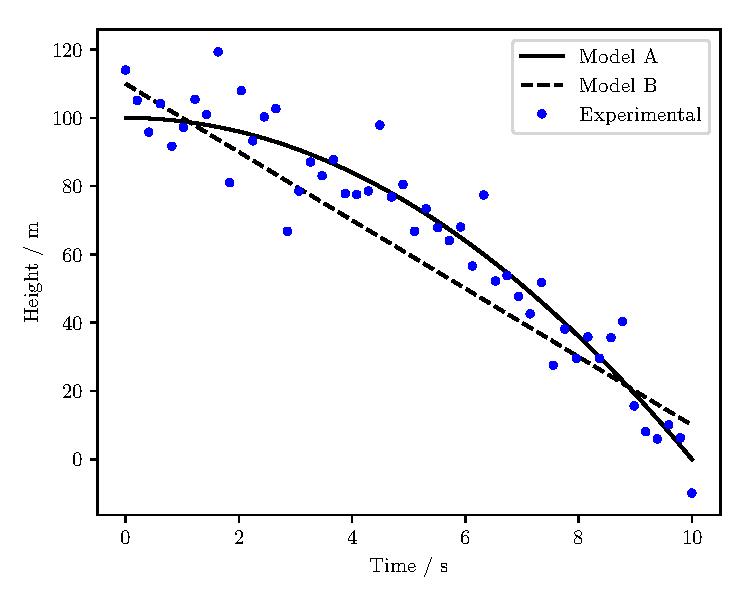
\includegraphics[width= 0.6\textwidth]{Figures/Height.pdf}
\caption[I don't have a list of figures]{Properly formatted graph.}
\label{fig:h-vs-t}
\end{figure}
\end{lstlisting}

\begin{figure}[!htbp]
\centering
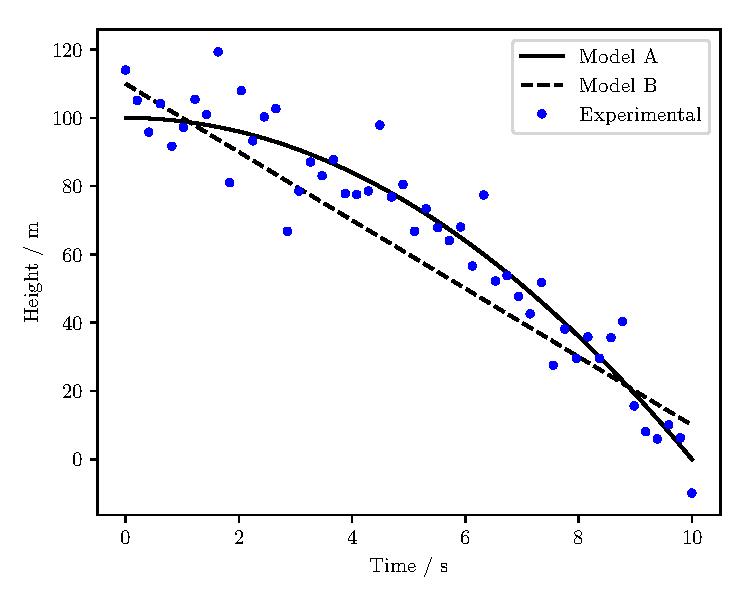
\includegraphics[width= 0.6\textwidth]{Figures/Height.pdf}
\caption[I don't have a list of figures]{Properly formatted graph.}
\label{fig:h-vs-t}
\end{figure}

The htbp refers to the placement of the figure in the order: here, top, bottom or next page. \LaTeX\ will do what it finds best, but adding an ! will force it to do what you say and not what it feels is best.

The centering command centre-aligns the figure. The third line is where the figure is actually inserted by using its filename as stated in the Figures subfolder. The square brackets are for command options; in this case the figure width is set to 60 \% of the text width. 

Likewise the caption has two parts. The caption in square brackets is what will be displayed in the list of figures (if needed) and the caption in curly brackets will be displayed below the figure. If these two are the same, you may simply leave out the square brackets. The label is the variable name for the figure and is used to reference the figure in-text \textit{eg}: $\backslash$ref\{fig:h-vs-t\}. The label name can be made anything, but \textsf{fig}, \textsf{fig} and \textsf{eq} are simply used to group the labels for similar objects together to find it easier in the suggestion box. In-text referencing is done by simply using the \texttt{ref} command. Precede it with a tilde for a nonbreaking space.



To insert two figures alongside each other, use a minipage environment. Two minipages are created in a figure environment with the width of each mini page less than 50 \% of the text width or else the figures will be below each other.

\begin{figure}[!htbp]
\centering
\begin{minipage}[t]{0.48\textwidth} 
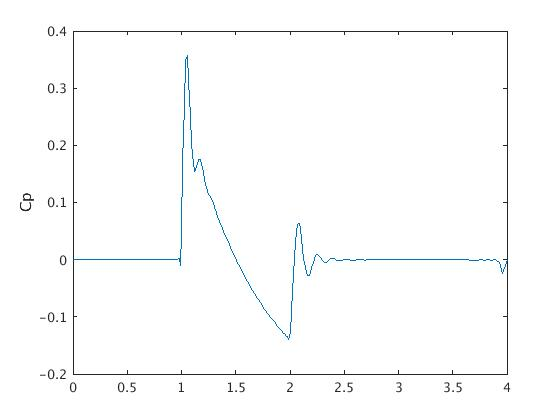
\includegraphics[width= \textwidth]{Figures/cp.jpg}
\caption{Pressure coefficient against airfoil.}
\label{fig:cp}
\end{minipage}
\begin{minipage}[t]{0.48\textwidth} 
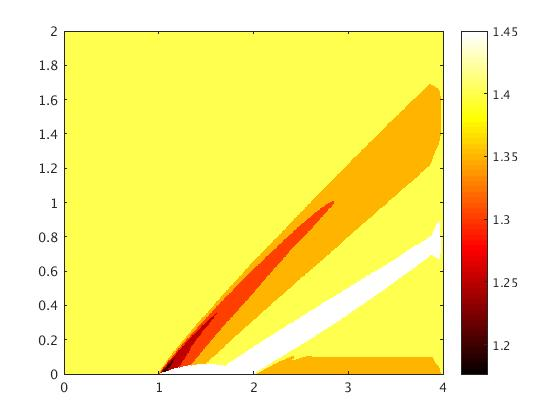
\includegraphics[width= \textwidth]{Figures/machcontour.jpg}
\caption{Mach number against the airfoil.}
\label{fig:mach}
\end{minipage}
\end{figure}    

\newpage
\subsection{Mathematics}
The excerpt below is to insert an equation:
\begin{lstlisting}
\begin{equation}
\dfrac{\partial \rho}{\partial t} + \nabla \cdot (\rho \bar{u}) = 0
\label{eq:continuity}
\end{equation}
\end{lstlisting}

For equations, Greek symbols can be entered by typing the name of the symbol (use a capital letter if an upper case letter is required). Refer to \href{https://www.sharelatex.com/learn/List_of_Greek_letters_and_math_symbols}{www.sharelatex.com} for more information on Greek and mathematical symbols. Consider Equation~\ref{eq:continuity}, Equation~\ref{eq:ftc}, and Equation~\ref{eq:taylor}

\begin{equation}
\label{eq:continuity}
\frac{\partial \rho}{\partial t} + \nabla \cdot (\rho \bar{u}) = 0
\end{equation}
\nomenclature{$\rho$}{Density (\si{\kilo \gram \per \cubic \meter})}
\nomenclature{$t$}{Time (\si{\second})}
\nomenclature{$u$}{Velocity (\si{\meter \per \second})}

\begin{equation}
\label{eq:ftc}
f(x) = \frac{\mathrm{d}}{\mathrm{d}x} \int^\infty_0  f(s) \, \mathrm{d}s
\end{equation}

\begin{equation}
\label{eq:taylor}
\sum^\infty_{n=0} \frac{f^{(n)}(a)}{n!} (x-a)^n
\end{equation}

Here are examples of chemical reactions

\begin{eqnarray*}
  \ce{A + 2B &<=>& AB2} \\
  \ce{MgCl_2 {\cdot} 6 H_2O &\xrightarrow{69 \; {\degree C}}& MgCl_2 {\cdot} 4 H_2O + 2H_2O} \\
\end{eqnarray*}

\subsection{Tables}
The main structure of the table is similar to that of a figure. Once again the code is enclosed by a begin and end command, a caption, and a label at the top. The excerpt below creates Table~\ref{tab:fpiorder}. The begin tabular command with three ls (lll) creates a table with left-aligned columns. The thicker top and bottom rules are made using the $\backslash$toprule and $\backslash$bottomrule commands. The thinner heading rule is made by using $\backslash$midrule. If you have a table of data from another program like Microsoft Excel, copy and paste them in the \href{https://www.tablesgenerator.com/}{\LaTeX{} Table Generator}.

\begin{lstlisting}
\begin{table}[!ht]
\centering
\caption{FPI rate and order of convergence}
\label{tab:fpiorder}
    \begin{tabular}{lll}
        \toprule
        k$_s$ & q & $\mu$ (cP) \\
        \midrule
        1 & 0.9940& -0.1761\\
        2 & 0.9887 & -0.2896\\
        4 & 0.9895& -0.4366\\
        \bottomrule
    \end{tabular}
\end{table}
\end{lstlisting}

\begin{table}[!ht]
    \centering
    \caption{FPI rate and order of convergence}
    \label{tab:fpiorder}
    \begin{tabular}{lll}
        \hlineB{3}
        k$_s$ (m s$^{-1}$) & q (W) & $\mu$ (cP) \\
        \midrule
        1 & 0.9940& -0.1761\\
        2 & 0.9887 & -0.2896\\
        4 & 0.9895& -0.4366\\
        \hlineB{3}  
    \end{tabular}
\end{table}

For a more advanced table, consider Table~\ref{tab:tabexample}.

\begin{table}[htbp]
  \centering
  \caption{Example of a table}
  \label{tab:tabexample}
  \begin{minipage}{0.5\textwidth}
    \begin{centering}
      \begin{tabular}{@{}llr@{}} \toprule 
        \multicolumn{2}{c}{Item}                                               \\ 
        \cmidrule(r){1-2} 
        Animal                    & Description & Price\textsuperscript{a} (R) \\ 
        \midrule 
        Gnat                      & per gram    & \num{13.65}                  \\ 
                                  & each        & \num{0.01}                   \\ 
        Parrot\textsuperscript{b} & stuffed     & \num{92.50}                  \\ 
        Emu                       & stuffed     & \num{33.33}                  \\ 
        Armadillo                 & frozen      & \num{8.99}                   \\ 
        \bottomrule 
      \end{tabular}                                                            \\
    \end{centering} 
    \vspace{1em}
    \textsuperscript{a} As of 2004                                             \\
    \textsuperscript{b} Norwegian blue only
  \end{minipage}
\end{table}

\subsection{Referencing}


When referencing literature, add your reference to the .bib file. To cite them in-text, use the commands in Table \ref{tab:Cite}.

\begin{table}[!ht]
\centering
\caption{In-text literature referencing examples}
\label{tab:Cite}
    \begin{tabular}{ll}
        \toprule
        \LaTeX\ syntax & Result\\
        \midrule
        $\backslash$parencite\{Bezuidenhoudt2017\} &\parencite{Bezuidenhoudt2017} \\
        $\backslash$textcite\{Bezuidenhoudt2017\} & \textcite{Bezuidenhoudt2017} \\
        $\backslash$parencite[250]\{Cengel2015\} &\parencite[250]{Cengel2015} \\
        $\backslash$textcite[250]\{Cengel2015\} & \textcite[250]{Cengel2015} \\
        \bottomrule
    \end{tabular}
\end{table}

This will create your reference list correct according to the departmental guidelines. Below is an example of a book and an article reference. For more examples see the \href{https://www.verbosus.com/bibtex-style-examples.html}{BibTeX Style Examples} website. 

\begin{lstlisting}
@Book{cengel2015,
  author		= {\c{C}engel, Y A and Ghajar, A J},
  title			= {Heat and Mass Transfer},
  publisher		= {McGraw-Hill},
  year			= 2015,
  address		= {New York},
  edition		= 5
}

@Article{Bezuidenhoudt2017,
  author   = {Bezuidenhoudt, A and Sonnendecker, PW and Crouse, PL},
  title	   = {Temperature and pressure effects on the product distribution of PTFE pyrolysis by means of qualitative, in-line FTIR analysis},
  journal  = {Polymer Degradation and Stability},
  year	   = 2017,
  pages	   = {79-88},
  volume   = {142}
}
\end{lstlisting}

To create a reference list at the end of your document, simply type: 
\begin{lstlisting}
\printbibliography
\end{lstlisting} 
\nocite{*}

\section{References}
\printbibliography[heading=none]
% \newpage
% \appendix
% \renewcommand{\thefigure}{\thesection.\arabic{figure}}
% \renewcommand{\thetable}{\thesection.\arabic{table}}
% \renewcommand{\thepage}{\thesection.\arabic{page}}
\end{document}